\begin{figure}[H]
    \centering
    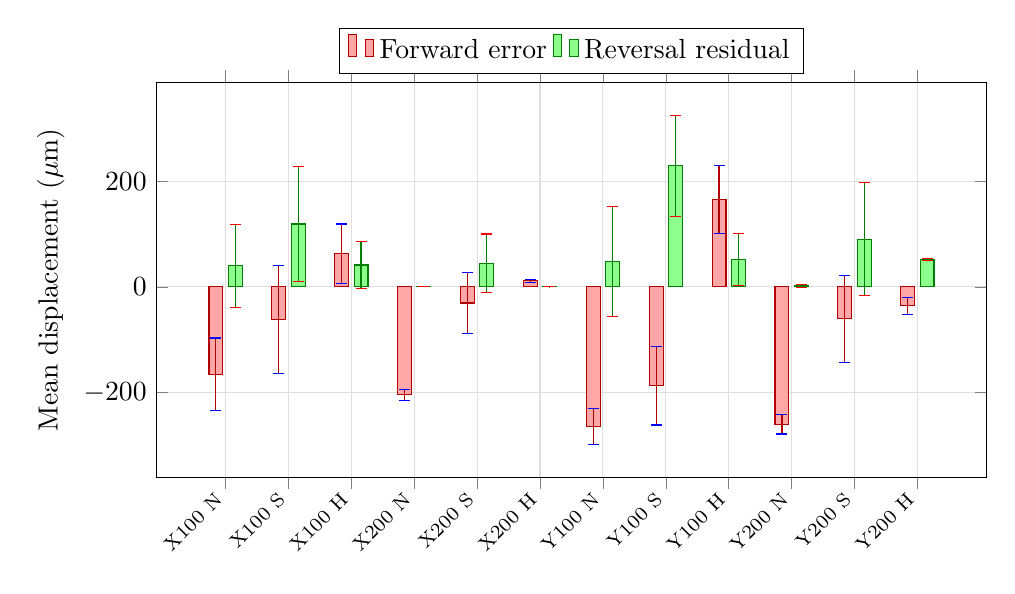
\begin{tikzpicture}
        \begin{axis}[
            width=\linewidth,
            height=6.6cm,
            ybar,
            bar width=5pt,
            ylabel={Mean displacement ($\mu$m)},
            symbolic x coords={X100N,X100S,X100H,X200N,X200S,X200H,Y100N,Y100S,Y100H,Y200N,Y200S,Y200H},
            xtick=data,
            xticklabels={X100 N,X100 S,X100 H,X200 N,X200 S,X200 H,Y100 N,Y100 S,Y100 H,Y200 N,Y200 S,Y200 H},
            x tick label style={rotate=45, anchor=east, font=\scriptsize},
            legend style={at={(0.5,1.02)}, anchor=south, legend columns=2},
            error bars/y dir=both, error bars/y explicit,
            grid=major,
            major grid style={draw=gray!25},
        ]
        \addplot+[fill=red!35, draw=red!70!black] coordinates {
            (X100N,-165.4447) +- (0,68.7159)
            (X100S,-61.7085) +- (0,102.2497)
            (X100H,63.2031) +- (0,56.0067)
            (X200N,-204.3472) +- (0,10.8359)
            (X200S,-30.3904) +- (0,58.4896)
            (X200H,11.4198) +- (0,2.8787)
            (Y100N,-264.7256) +- (0,33.6487)
            (Y100S,-186.9259) +- (0,74.6672)
            (Y100H,165.4600) +- (0,63.9804)
            (Y200N,-260.0961) +- (0,18.4527)
            (Y200S,-60.6364) +- (0,83.0260)
            (Y200H,-35.8059) +- (0,16.3546)
        };
        \addlegendentry{Forward error}
        \addplot+[fill=green!45, draw=green!50!black] coordinates {
            (X100N,40.0263) +- (0,78.7283)
            (X100S,119.1569) +- (0,109.5918)
            (X100H,41.4716) +- (0,45.0833)
            (X200N,0.8661) +- (0,0.6902)
            (X200S,44.7546) +- (0,55.4842)
            (X200H,0.2663) +- (0,0.1992)
            (Y100N,48.3540) +- (0,104.4839)
            (Y100S,229.3735) +- (0,96.1114)
            (Y100H,51.6279) +- (0,49.4374)
            (Y200N,2.0957) +- (0,2.8116)
            (Y200S,90.3723) +- (0,107.4034)
            (Y200H,52.5853) +- (0,1.7197)
        };
        \addlegendentry{Reversal residual}
        \end{axis}
    \end{tikzpicture}
    \caption[4x motion-accuracy results]{Motion-accuracy results on a 4x objective. Forward error compares measured displacement with the commanded displacement. Reversal residual is the remaining image offset after returning. Error bars show one standard deviation. Labels combine axis, commanded step count, and mode: N=No compensation, S=Sign compensation, H=Hysteresis compensation.}
    \label{fig:eval-motion}
\end{figure}
